%!TEX TS-program = XeLaTeX
\documentclass[11pt]{article}

\usepackage{amssymb}
\usepackage{amsthm}
\usepackage{amsmath}
\usepackage{mathtools}

\usepackage{fancyhdr}
\usepackage{graphicx}
\usepackage[top=3cm, left=2cm, right=2cm, headheight = 90pt]{geometry}
\usepackage{xltxtra}
\usepackage[font=small,labelfont=bf]{caption}

%%%%%%%%%%%%%%    Language matters  %%%%

%\usepackage[latvian]{babel}
%\usepackage[L7x]{fontenc}
%\usepackage[utf8x]{inputenc}

%%%%%%%%%%%%%%%%%%%%%%%%%%%%%%%%%%%7%%%%%

%%%%%%%%%%%%%%%%%%%%%%%%%%%       DO NOT EDIT         %%%%%%%%%%%%%%%%%%
%\usepackage{space}
%\renewcommand{\headrulewidth}{1pt}
%\fancyhead[L]{\includegraphics[width=3cm]{pictures/logo}}
%\fancyhead[R]{\raisebox{3ex}{\fbox{Language: \bf \lang}}}
\fancyhead[C]{{\Large\bf Indukcija - Uzdevumi}\\ \date}

\renewcommand{\theenumi}{\alph{enumi}}
%\newcommand{\problem}[1]{\paragraph{Problem #1.}}%<--------------- TRANSLATE THE WORD "Problem".
\fancyfoot[CE,CO]{}  % this is to remove page numbers (as you might want for single page docs)

\def\leq{\leqslant}
\def\geq{\geqslant}
\def\N{\mathbb N}
\def\R{\mathbb R}
\def\Z{\mathbb Z}
\DeclarePairedDelimiter\set\{\}
\newcommand{\?}{\stackrel{?}{=}}

%%%%%%%%%%%%%%%%%%%%%%%%%%%%%%%%%%%%%%%%%%%%%%%%%%%%%%%%%%%%%%%%%%%%%%%%%


%%% Language name in english %%%%%%%%%
\def\lang{Latvian}

%\def\lang{Lithuanian}

%%%%%%%%%%%%%%%%%%%%%%%%%%%%% TRANSLATE HERE %%%%%%%%%%%%%%%%%%%%%%%%%%%%%%%%%%

%\def\date{2018. gada 18. jūnijs}
%\def\notes{}


%%%%%%%%%%%%%%%%%%%%%%%%%%%%%%%%%%%%%%%%%%%%%%%%%%%%%%%%%%%%%%%%%%%%%%%%%%%%%%%

\def\prob{}

%%%%%%%%%%%%%%%%%%%%%%%%%%%%%%%%%%%%%%%%%%%%%%%%%%%%%%%%

\theoremstyle{definition}
\newtheorem{problem}{\prob}
\renewcommand{\figurename}{Attēls}

\pagestyle{fancy}



\begin{document}
%\thispagestyle{fancy}
\noindent 
%\emph{\notes}

%1
\begin{problem}
\textit{[Sienāzīša indukcija]}
Nemirstīgs sienāzītis sēž uz bezgalīgu kāpņu pirmā pakāpiena. Sienāzītis ir spējīgs uzņemt visuma enerģiju ar ātrumu, kas ļauj viņam reizi minūtē pārlēkt no viena pakāpiena uz nākamo.

Pierādiet, ka sienāzītis spēs sasniegt savu mīļāko zvaigzni, lai cik tālu tā arī neatrastos!

\end{problem}
%

%2
\begin{problem}
\textit{[Kāpuriņa indukcija]}
Bezgalīgi garš kāpurs ir pierāpojis pie bezgalīgajām kāpnēm uz pamanījies uzsliet galvu un priekškājas(?) uz pirmajiem diviem pakāpieniem. Zināms, ka, ja kāpurs atbalstās uz pirmajiem $k$ pakāpieniem, tad viņš var uzspiest sevi arī uz $k+1$. pakāpiena.

Pierādiet, ka arī kāpurs var sasniegt sienāzīša mīļāko zvaigzni!
\end{problem}
%

%3
\begin{problem}
\textit{[Trīsstūraini skaitļi]}
Skaitli $T$ sauc par \textit{trīsstūrainu}, ja $T$ punktus var izkārtot vienādmalu trīsstūra piramīdā tā, ka katrā līmenī ir par vienu punktu vairāk, nekā iepriekšējā. Pirmie trīsstūrveida skaitļi ir:
\begin{center}
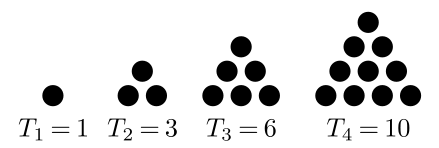
\includegraphics[width=5cm]{Triangular_numbers.png}
\captionof{figure}{Pirmie trīsstūrveida skaitļi}
\label{fig:TriangularNumbers}
\end{center}

Pierādiet, ka $T_n=\frac{n(n+1)}{2}$!
\end{problem}
%

%4
\begin{problem}
\textit{[Slapja padarīšana]}
Uz galda stāv $128$ vienādas glāzes, bet katrā ir ieliets dažāds daudzums ūdens. Pēterītis prot paņemt jebkuras divas glāzes un liet no vienas otrā, kamēr ūdens daudzums abās ir vienāds.

Pierādiet, ka Pēterītis var panākt, ka visās glāzēs uz galda ir vienāds ūdens daudzums!
\end{problem}
%


%5
\begin{problem}
\textit{[Pilna Vienvirziena zeme]}
Vienvirziena zemē katra pilsēta ir savienota ar katru citu ar vienu vienvirziena ceļu. 

Pierādiet, ka Vienvirziena zemē ir pilsēta no kuras var nonākt jebukā citā pilsētā!
\end{problem}
%


%6
\begin{problem}
\textit{[Daļēja Vienvirziena zeme]}
Šajā Vienvirziena zemē tikai dažas pilsētas ir savienotas ar kādām citām ar vienvirziena ceļu (un nav pilnībā nesavienotu daļu). Tapat ir zināms, ka, katrai pilsētai ceļu skaits, kas iziet no tās, ir vienāds ar ceļu skaitu, kas tajā ieiet. 

Pierādiet, ka šajā Vienvirziena zemē no katras pilsētas ir iespējams nonākt katrā citā!
\end{problem}
%

%7
\begin{problem}
\textit{[Atkal Pilna Vienvirziena zeme]}
Mēs atkal esam Pilnā Vienvirziena zemē, kurā katra pilsēta ir savienota ar katru (ar vienvirziena ceļu). 

Pierādiet, ka, ja šajā zemē ir vismaz $3$ pilsētas, tad ir iespējams nomainīt maksimums viena ceļa virzienu tā, ka pēc tam būs iespējams no katras pilsētas nonākt jebkurā citā!
\end{problem}
%

%8
\begin{problem}
\textit{[Kvadrāta pārklāšana ar stūrīšiem]}
Kāds no $128\times128$ rūtiņu kvadrāta ir izgriezis vienu rūtiņu. 

Pierādiet, ka atlikušo kvadrāta daļu var noklāt ar "stūrīšiem"!
\begin{center}
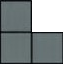
\includegraphics[width=0.7cm]{corner.png}
\captionof{figure}{Stūrītis}
\label{fig:Coner}
\end{center}
\end{problem}
%

%9
\begin{problem}
\textit{[Lapsiņas problēma]}
$100$ trusīšu mežā atrada mellenes. Jaunākais trusītis salasīja $1$ melleni, otrs jaunākais - $2$ mellenes, trešais - $4$ mellenes un tā tālāk līdz vecākais salasīja $2^{99}$ mellenes. 
Pienāca lapsiņa un piedāvājās palīdzēt pārdalīt ogas godīgāk - viņa atkārtoti izvēlēsies divus trusīšus un sadalīs viņu kopīgo ogu skaitu starp viņiem līdzīgi, pati apēdot lieko ogu (ja kopskaits ir nepāra) kā samaksu par darbu. 

Kāds ir lielākais skaits melleņu, ko lapsiņa var apēst ar šādiem noteikumiem?
\end{problem}
%

%10
\begin{problem}
\textit{[Atkal kliķes]}
Grupā ir $n$ cilvēku, no kuriem daži ir abpusēji pazīstami. $i$-tā cilvēka paziņu skaitu apzīmēsim ar $d_i$. Pierādiet, ka šajā grupā ir vismaz $$\sum_{i=1}^{n}{\frac{1}{d_i +1}}$$ savstarpēji nepazīstamu cilvēku.
\end{problem}
%

%11 IMO2006 SLC1
\begin{problem}
\textit{[Spundžu slēgāšana]}

Mums ir rinda ar $n \ge 2$ lamps $L_1, \dots, L_n$ spuldzes, katra no tām var būt ieslēgta vai izslēgta. Katru sekundi mēs vienlaicīgi mainam visu spuldžu stāvokli pēc sekojošiem noteikumiem:
\begin {itemize}
\item ja spuldzīte $L_i$ un visi tās kaimiņi (pirmajai un pēdējai spuldzītei ir viens kaimiņš, pārējām - divi) ir vienā stāvoklī, tad $L_i$ tiek izslēgta;
\item citādi, $L_i$ tiek ieslēgta.
\end {itemize}
Sākumā visas spuldzītes ir izslēgtas, izņemot pašu pirmo, kura ir ieslēgta.
\begin {enumerate}
\item Pierādiet, ka ir bezgalīgi daudz $n$ vērtību, kurām kādā brīdī visas spuldzītes būs izslēgtas. 
\item Pierādiet, ka ir bezgalīgi daudz $n$ vērtību, kurām visas spuldzītes nekad būs vienlaicīgi izslēgtas. 
\end {enumerate}

\end{problem}
%

%12 IMO2005 SLC5
\begin{problem}
\textit{[Monētu grozīšana]}

Rindā sakārtotas $n$ monētas, kurām katrai ir balta un melna puse. Sākumā visas monētas novietotas ar bato pusi uz augšu. 
Katrā gājienā, ja vien tas ir iespējams, mēs izvēlamies monētu ar balto pusi uz augšu (bet ne vienu no pašām malējām monētām), to novācam un apgriešam otrādi tai blakusstāvošās monētas. Kādiem $n$ iespējams panākt, ka kādā brīdī iegūsim tikai divas monētas?


\end{problem}
%
\end{document}
